%
%Не забыть:
%--------------------------------------
%Вставить колонтитулы, поменять название на титульнике



%--------------------------------------

\documentclass[a4paper, 12pt]{article} 

%--------------------------------------
%Russian-specific packages
%--------------------------------------
%\usepackage[warn]{mathtext}
\usepackage[T2A]{fontenc}
\usepackage[utf8]{inputenc}
\usepackage[english,russian]{babel}
\usepackage[intlimits]{amsmath}
\usepackage{esint}
%--------------------------------------
%Hyphenation rules
%--------------------------------------
\usepackage{hyphenat}
\hyphenation{ма-те-ма-ти-ка вос-ста-нав-ли-вать}
%--------------------------------------
%Packages
%--------------------------------------
\usepackage{amsmath}
\usepackage{amssymb}
\usepackage{amsfonts}
\usepackage{amsthm}
\usepackage{latexsym}
\usepackage{mathtools}
\usepackage{etoolbox}%Булевые операторы
\usepackage{extsizes}%Выставление произвольного шрифта в \documentclass
\usepackage{geometry}%Разметка листа
\usepackage{indentfirst}
\usepackage{wrapfig}%Создание обтекаемых текстом объектов
\usepackage{fancyhdr}%Создание колонтитулов
\usepackage{setspace}%Настройка интерлиньяжа
\usepackage{lastpage}%Вывод номера последней страницы в документе, \lastpage
\usepackage{soul}%Изменение параметров начертания
\usepackage{hyperref}%Две строчки с настройкой гиперссылок внутри получаеммого
\usepackage[usenames,dvipsnames,svgnames,table,rgb]{xcolor}% pdf-документа
\usepackage{multicol}%Позволяет писать текст в несколько колонок
\usepackage{cite}%Работа с библиографией
\usepackage{subfigure}% Человеческая вставка нескольких картинок
\usepackage{tikz}%Рисование рисунков
\usepackage{float}% Возможность ставить H в положениях картинки
% Для картинок Моти
\usepackage{misccorr}
\usepackage{lscape}
\usepackage{cmap}



\usepackage{graphicx,xcolor}
\graphicspath{{Pictures/}}
\DeclareGraphicsExtensions{.pdf,.png,.jpg}

%----------------------------------------
%Список окружений
%----------------------------------------
\newenvironment {theor}[2]
{\smallskip \par \textbf{#1.} \textit{#2}  \par $\blacktriangleleft$}
{\flushright{$\blacktriangleright$} \medskip \par} %лемма/теорема с доказательством
\newenvironment {proofn}
{\par $\blacktriangleleft$}
{$\blacktriangleright$ \par} %доказательство
%----------------------------------------
%Список команд
%----------------------------------------
\newcommand{\grad}
{\mathop{\mathrm{grad}}\nolimits\,} %градиент

\newcommand{\diver}
{\mathop{\mathrm{div}}\nolimits\,} %дивергенция

\newcommand{\rot}
{\ensuremath{\mathrm{rot}}\,}

\newcommand{\Def}[1]
{\underline{\textbf{#1}}} %определение

\newcommand{\RN}[1]
{\MakeUppercase{\romannumeral #1}} %римские цифры

\newcommand {\theornp}[2]
{\textbf{#1.} \textit{ #2} \par} %Написание леммы/теоремы без доказательства

\newcommand{\qrq}
{\ensuremath{\quad \Rightarrow \quad}} %Человеческий знак следствия

\newcommand{\qlrq}
{\ensuremath{\quad \Leftrightarrow \quad}} %Человеческий знак равносильности

\renewcommand{\phi}{\varphi} %Нормальный знак фи

\newcommand{\me}
{\ensuremath{\mathbb{E}}}

\newcommand{\md}
{\ensuremath{\mathbb{D}}}



%\renewcommand{\vec}{\overline}




%----------------------------------------
%Разметка листа
%----------------------------------------
\geometry{top = 3cm}
\geometry{bottom = 2cm}
\geometry{left = 1.5cm}
\geometry{right = 1.5cm}
%----------------------------------------
%Колонтитулы
%----------------------------------------
\pagestyle{fancy}%Создание колонтитулов
\fancyhead{}
%\fancyfoot{}
\fancyhead[R]{\textsc{Изучение поляризованного света}}%Вставить колонтитул сюда
%----------------------------------------
%Интерлиньяж (расстояния между строчками)
%----------------------------------------
%\onehalfspacing -- интерлиньяж 1.5
%\doublespacing -- интерлиньяж 2
%----------------------------------------
%Настройка гиперссылок
%----------------------------------------
\hypersetup{				% Гиперссылки
	unicode=true,           % русские буквы в раздела PDF
	pdftitle={Заголовок},   % Заголовок
	pdfauthor={Автор},      % Автор
	pdfsubject={Тема},      % Тема
	pdfcreator={Создатель}, % Создатель
	pdfproducer={Производитель}, % Производитель
	pdfkeywords={keyword1} {key2} {key3}, % Ключевые слова
	colorlinks=true,       	% false: ссылки в рамках; true: цветные ссылки
	linkcolor=blue,          % внутренние ссылки
	citecolor=blue,        % на библиографию
	filecolor=magenta,      % на файлы
	urlcolor=cyan           % на URL
}
%----------------------------------------
%Работа с библиографией (как бич)
%----------------------------------------
\renewcommand{\refname}{Список литературы}%Изменение названия списка литературы для article
%\renewcommand{\bibname}{Список литературы}%Изменение названия списка литературы для book и report
%----------------------------------------
\begin{document}
	\begin{titlepage}
		\begin{center}
			$$$$
			$$$$
			$$$$
			$$$$
			{\Large{НАЦИОНАЛЬНЫЙ ИССЛЕДОВАТЕЛЬСКИЙ УНИВЕРСИТЕТ}}\\
			\vspace{0.1cm}
			{\Large{ВЫСШАЯ ШКОЛА ЭКОНОМИКИ}}\\
			\vspace{0.25cm}
			{\large{Факультет физики}}\\
			\vspace{5.5cm}
			{\Huge\textbf{{Лабораторная работа}}}\\%Общее название
			\vspace{1cm}
			{\LARGE{<<Изучение поляризованного света>>}}\\%Точное название
			\vspace{2cm}
			{Работу выполнил студент 3 курса}\\
			{Захаров Сергей Дмитриевич}
			\vfill
			
\includegraphics[width = 0.2\textwidth]{HSElogo}\\
			\vfill
			Москва\\
			2020
		\end{center}
	\end{titlepage}
	
\tableofcontents

\newpage

\section{Цели работы}

Перед началом работы были поставлены следующие задачи:

\begin{enumerate}
	\item Определить поляризацию света от лазера.
	
	\item Экспериментально проверить закон Малюса.
	
	\item Определить главные направления пластинок $\lambda/2$ и $\lambda/4$ по отношению к входному поляризатору. Определить поляризацию прошедшего света.
	
	\item Определить тип неизвестной пластинки.
	
	\item Определить угол Брюстера для темного стекла. Определить его показатель преломления.
	
	\item Экспериментально проверить формулы Френеля.
\end{enumerate}

\section{Порядок выполнения работы}

\subsection{Определение поляризации света от источника}

Для того, чтобы определить поляризацию света, на пути света от источника был установлен поляризатор, после чего начали вращать последний. Если бы у света была круговая поляризация, то значение интенсивности бы от этого не менялось; если бы поляризация была чисто линейной, то минимальное значение интенсивности оказалось бы равным нулю. В реальности же были получены следующие значения:

\begin{align*}
	& I_{max} = 493 \text{ $\mu$Вт} \\
	& I_{min} = 239 \text{ $\mu$Вт}
\end{align*}

Исходя из этого сделаем вывод, что свет от лазера имеет линейную + естественную поляризацию.

\subsection{Проверка справедливости закона Малюса}

Для проверки справедливости указанного закона, после уже установленного поляризатора был установлен еще один. Из-за того, что после поляризатора получается линейно поляризованный свет, становится возможным определить положение второго поляризатора, при котором его главное направление совпадает с главным направление первого, просто определив, при каком положении достигается максимум интенсивности проходящего света. Затем, для подтверждения закона Малюса, достаточно постепенно увеличивать угол между главными направлениями, что и было сделано.

Результаты измерений можно увидеть на графике. Видно, что они в целом соответствуют предсказанным согласно закону Малюса значениям:

\begin{equation}
		I = I_0 \cos^2\Delta\alpha
		\label{eq:malus_law}
\end{equation}

Результаты измерений приведены на графике (\ref{fig:malus}).

\begin{figure}[H]
	\centering
	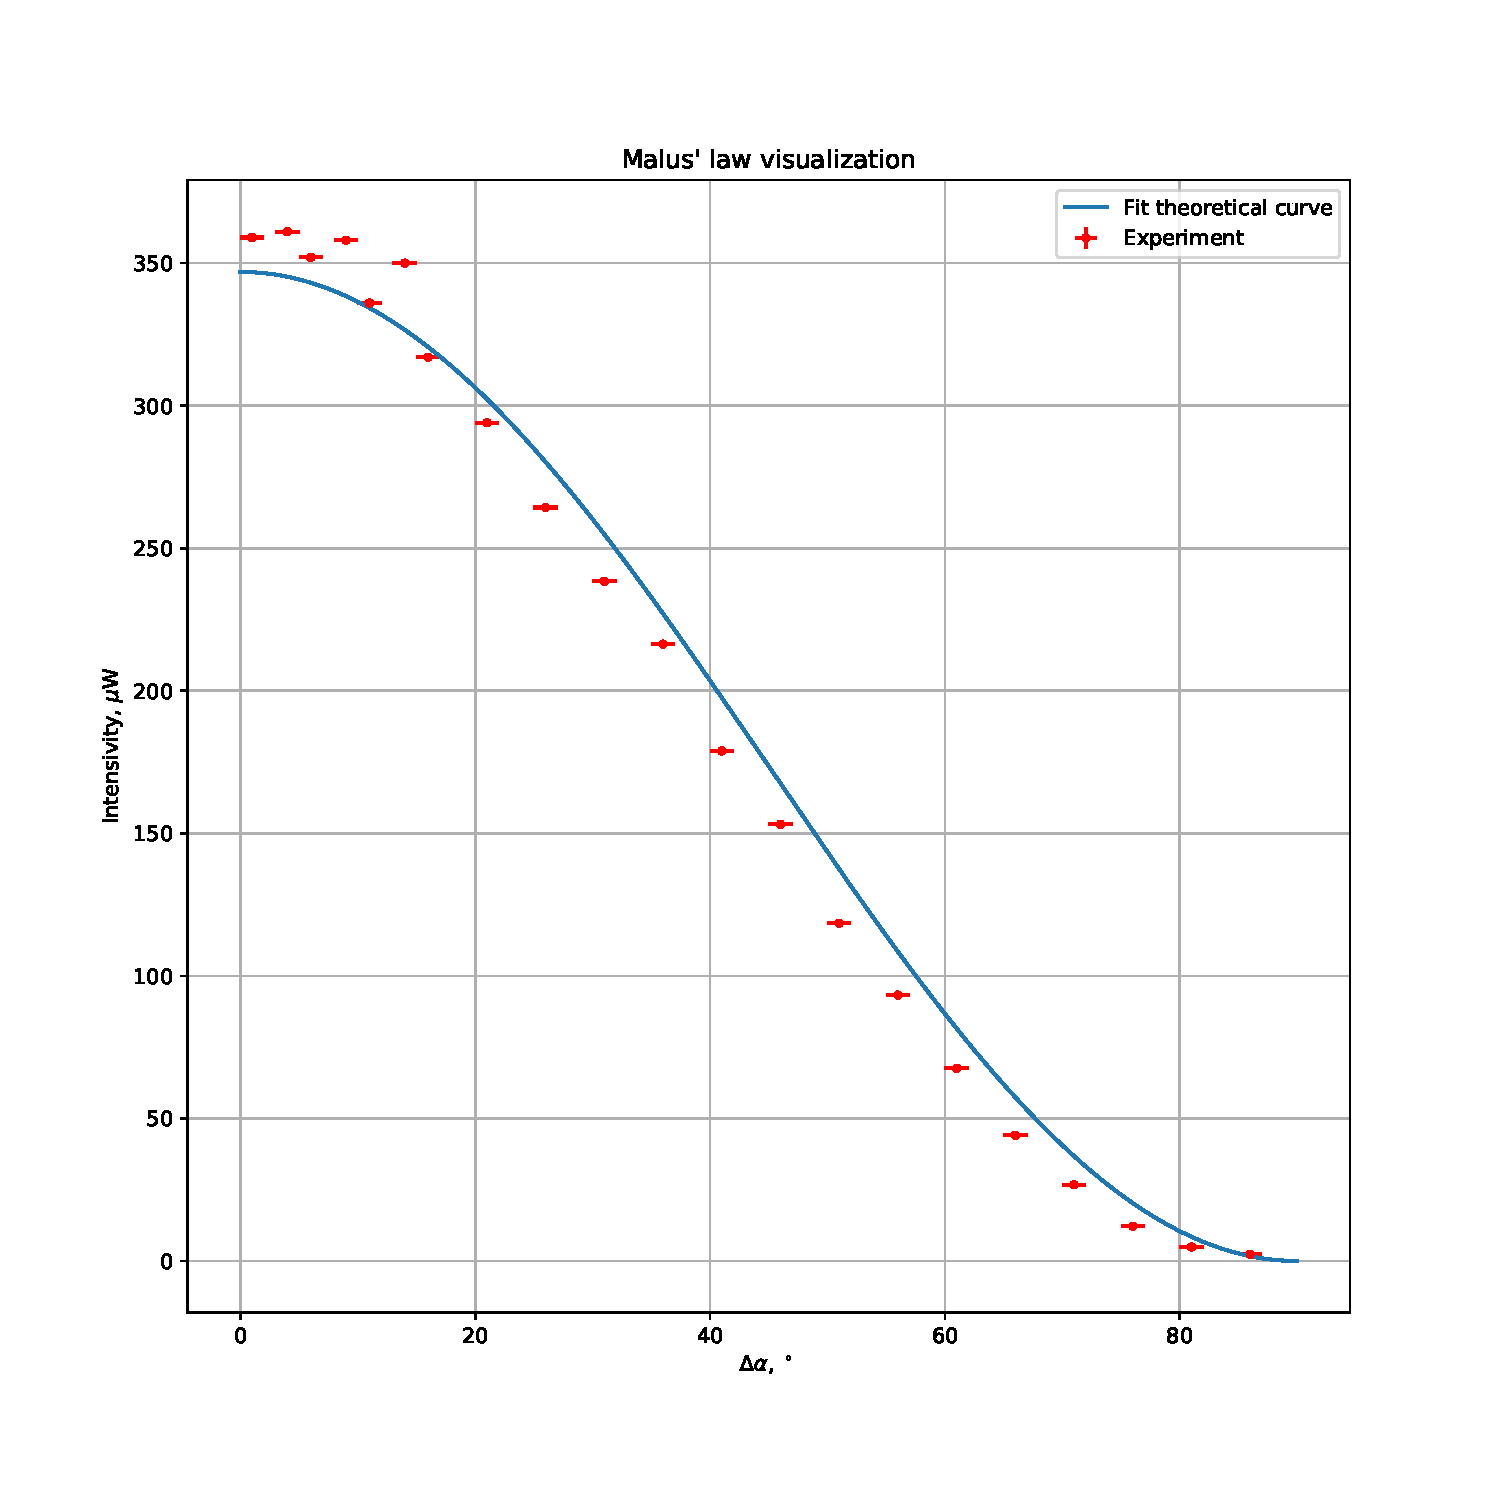
\includegraphics[width=\linewidth]{lab_1}
	\caption{Зависимость интенсивности проходящего света от угла между главными направлениями поляризаторов (иллюстрация закона Малюса).}
	\label{fig:malus}
\end{figure}

\subsection{Определение главного направления пластинок $\lambda / 4$ и $\lambda / 2$ по отношению к входному поляризатору}

Чтобы определить главное направление пластинок, второй поляризатор был установлен таким образом, чтобы оказаться скрещенным с первым. В таком случае (в идеальной ситуации) интенсивность света, падающего на измеритель интенсивности, оказывается равной нулю.

При работе с пластинкой $\lambda / 2$, если ее главное направление оказывается под углом $45^\circ$ к направлению поляризации линейно поляризованного света, то направление поляризации изменится на $90^\circ$. В таком случае, при прохождении второго поляризатора мы увидим максимум интенсивности. Именно это и было сделано и именно это и получилось пронаблюдать.

Это подтверждается следующими минимальными и максимальными значениями интенсивности:

\begin{align*}
	&I_{max} = 281 \pm 0.1 \text{ $\mu$Вт}\\
	&I_{min} = 5.27 \pm 0.1 \text{ $\mu$Вт}\\
\end{align*}

При работе же с четвертьволновой пластинкой, при тех же условиях, поляризация света переходит в круговую. В таком случае, при повороте второго поляризатора, интенсивность света, проходящего через него, не должна изменяться. Это подтверждается и наблюдениями:

\begin{align*}
	&I_{max} = 174 \pm 0.1 \text{ $\mu$Вт}\\
	&I_{min} = 158 \pm 0.1 \text{ $\mu$Вт}\\
\end{align*}

\subsection{Определение типа ($\lambda/2$ или $\lambda/4$) неизвестной пластинки}

Для того, чтобы определить тип пластинки, можно воспользоваться методами, изложенными выше. Путем последовательных поворотов пластинки, мы убедились, что перед нами пластинка $\lambda/2$. Это становится ясно, если увидеть минимальные и максимальные значения интенсивности (при условии, что поляризаторы были скрещены):

\begin{align*}
	&I_{max} = 300 \pm 0.1 \text{ $\mu$Вт}\\
	&I_{min} = 17.3 \pm 0.1 \text{ $\mu$Вт}\\
\end{align*}

\subsection{Определение величины угла Брюстера пластинки и проверка справедливости формул Френеля}

Для того, чтобы определить угол Брюстера, необходимо определить, при каком угле падения и положении поляризатора достигается минимальная интенсивность отраженного света (который поляризован линейно после прохождения поляризатора). Эта ситуация будет соответствовать углу падения, равному углу Брюстера, а поляризация будет соответствовать случаю $p$-поляризации.

В результате угол Брюстера оказался равен:

\begin{equation*}
		\theta_{B} = 60 \pm 0.5 ^\circ 
\end{equation*}

Отсюда несложно сделать вывод о показателе преломления вещества:

\begin{equation*}
		n = \tan\theta_B \approx 1.73 \pm 0.11
\end{equation*}

Чтобы проверить формулы Френеля, достаточно, не меняя положения поляризатора (чтобы не менять $p$-поляризацию), изменить угол падения. После этого (для проверки второй формулы для $s$-поляризации), необходимо повернуть поляризатор на 90$^\circ$, чтобы поменять поляризацию на $s$-поляризацию, и сделать то же самое, после чего сравнить их с результатами, полученными с помощью упомянутых формул Френеля:

\begin{align}
	I_{rs} = \left|\frac{n_1\cos\alpha - n_2\cos\gamma}{n_1\cos\alpha + n_2 \cos\gamma}\right|^2 I_0\\
	I_{rp} = \left|\frac{n_1\cos\gamma - n_2\cos\alpha}{n_1\cos\gamma + n_2\cos\alpha}\right|^2 I_0
	\label{eq:fresnel}
\end{align}

В данном случае мы можем с достаточной точностью сказать, что $n_1 = 1$, а $\cos\gamma$ можно найти по формуле Снеллиуса:

\begin{equation}
	n_1\sin\alpha = n_2\sin\gamma
	\label{eq:snel}
\end{equation}

С учетом всего вышесказанного, в ходе работы был получен следующий график:

\begin{figure}[H]
	\centering
	\subfigure[]{
		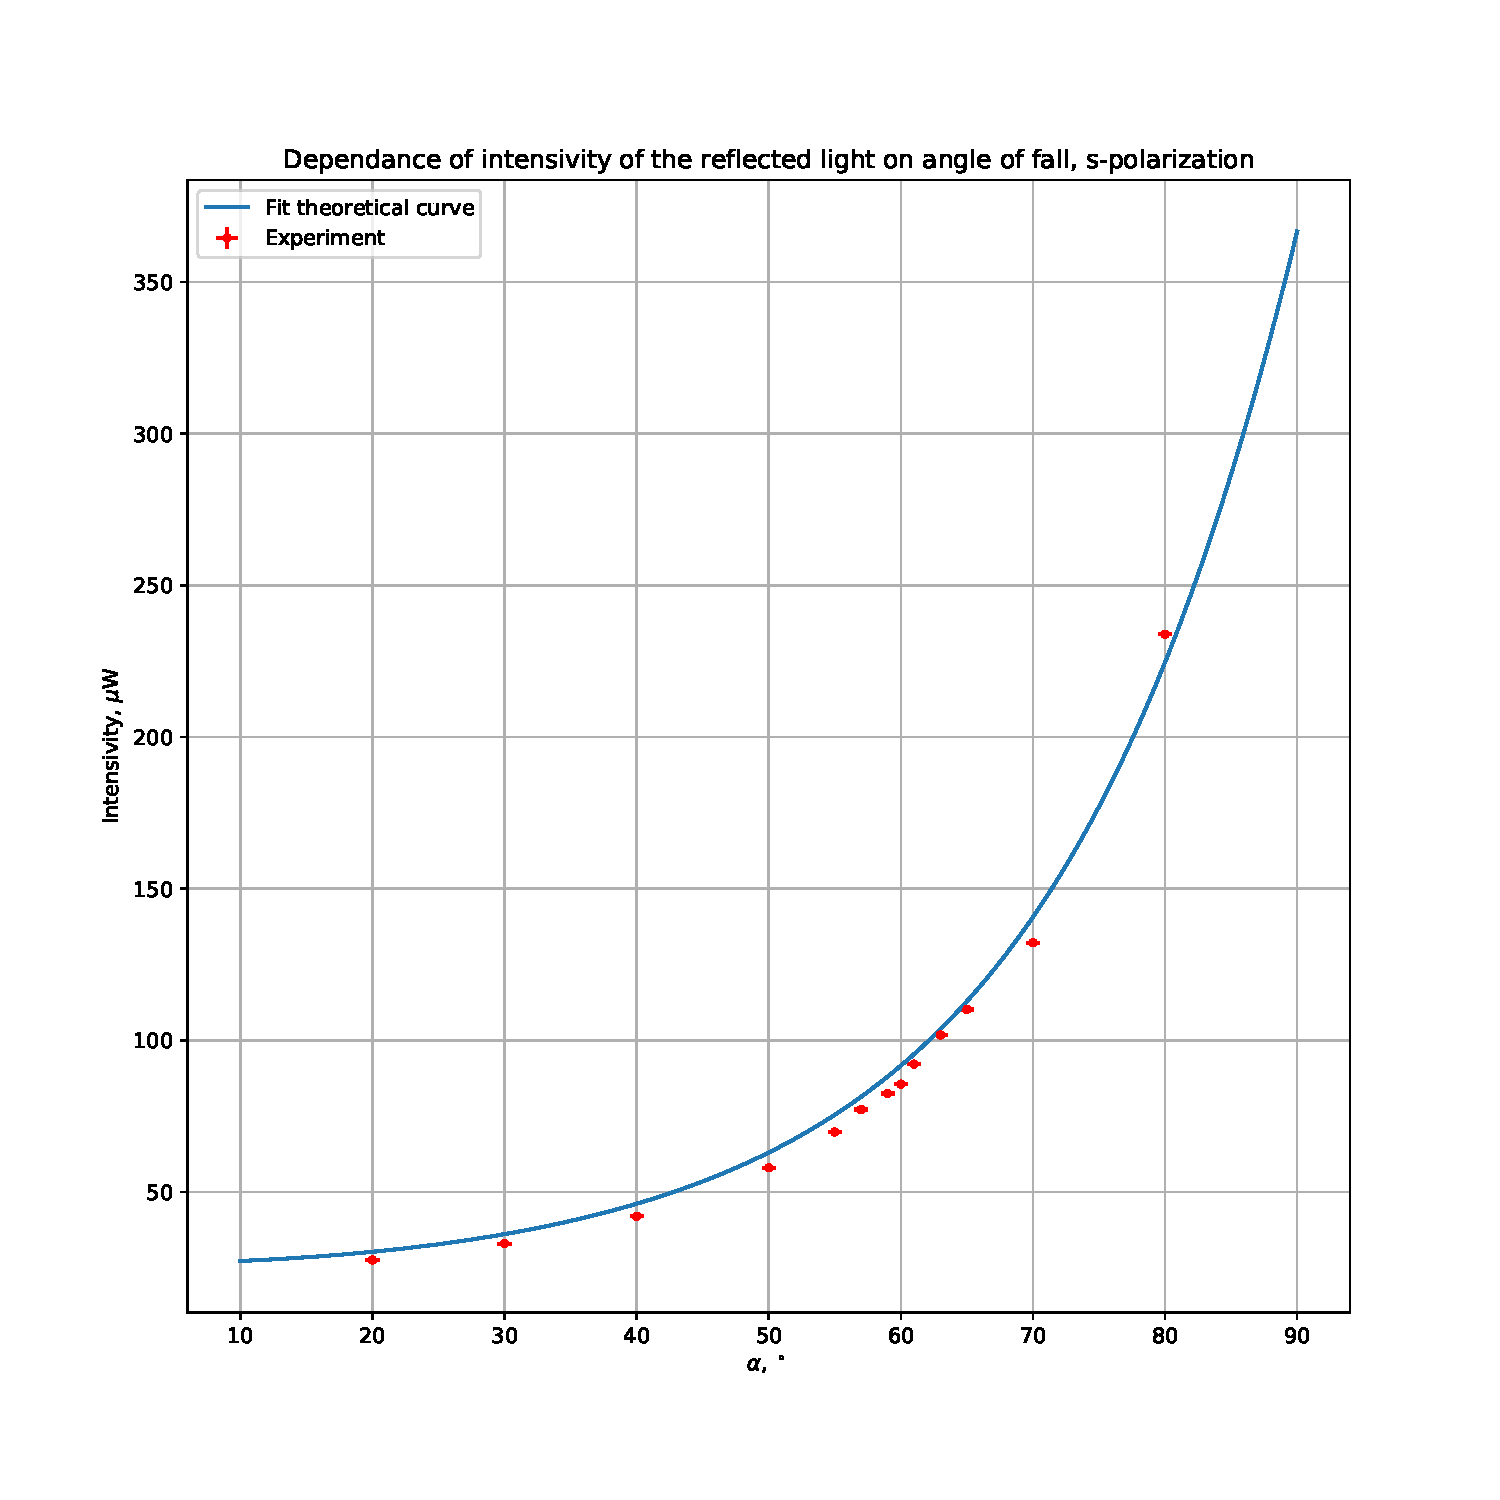
\includegraphics[width=0.48\linewidth]{lab_2_1}	
	}
	\subfigure[]{
		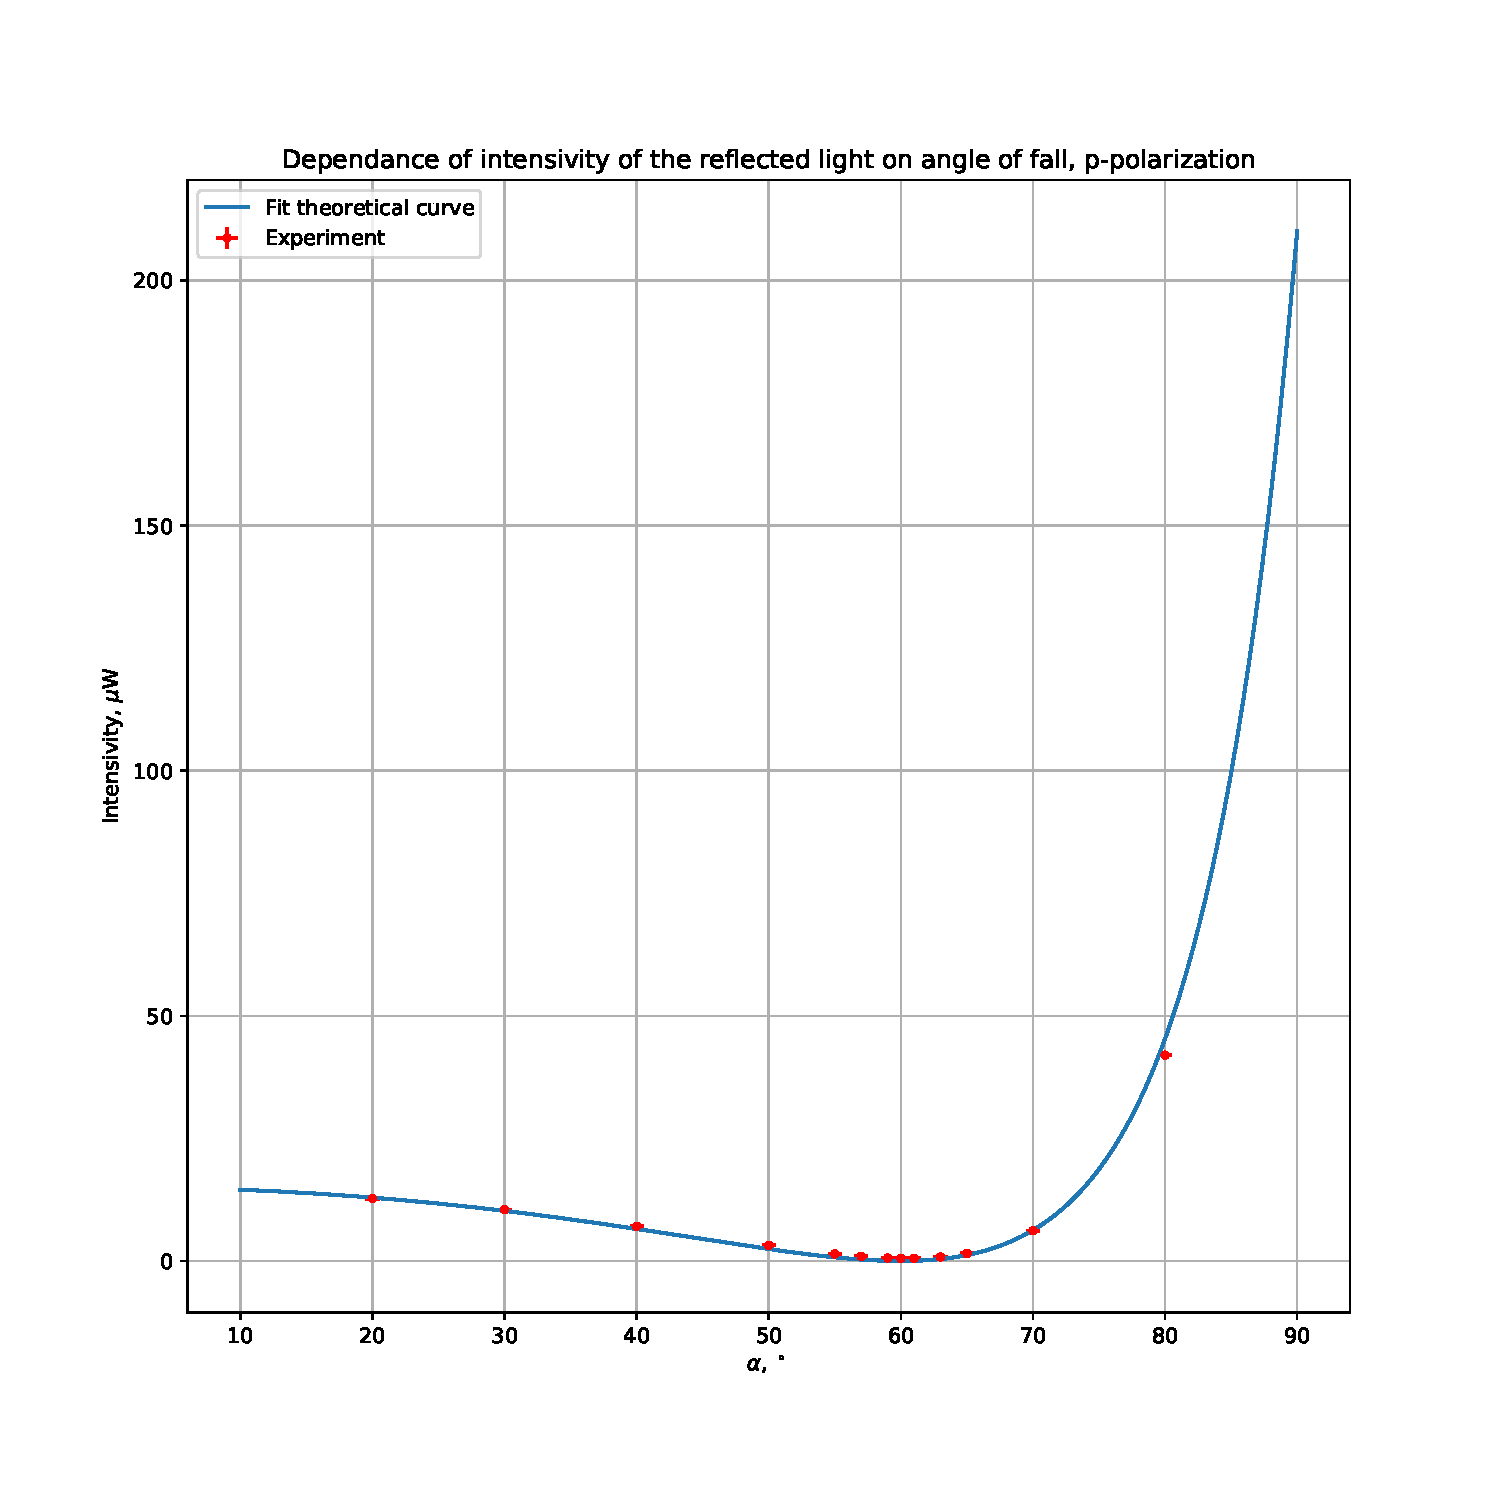
\includegraphics[width=0.48\linewidth]{lab_2_2}
	}
	\caption{Зависимость интенсивности отраженного света от угла падения на затемненное стекло в случае (a) $s$-поляризации (b) $p$-поляризации.}
\end{figure}

\section{Выводы}

\begin{enumerate}
	\item В ходе работы было определено, что излучение от лазера имеет преимущественно линейную поляризацию с примесью естественного света.
	
	\item Был экспериментально подтвержден закон Малюса.
	
	\item Экспериментально были определены главные направления полуволновой и четвертьволновой пластинок. Кроме того, были определены поляризации света после прохождения каждой из пластин.
	
	\item Было экспериментально установлено, что неизвестная пластинка является полуволновой пластинкой.
	
	\item Был определен угол Брюстера для предложенного темного стекла: $\theta_{B}=60\pm0.5^\circ$. Исходя из этого, был вычислен показатель преломления стекла: $n \approx 1.73 \pm 0.11$.
	
	\item Наконец, были экспериментально подтверждены формулы Френеля.
\end{enumerate}






\end{document}